\documentclass{./../../Latex/tests}

\begin{document}
\thispagestyle{plain}
\myheader{Final Exam Sample}
\rhead{Final Exam Sample}
\vspace{0.5em}
\testHeader{90}{20}

\begin{enumerate}
\item (6 pts) Multiple-choice questions 
\begin{enumerate}
\item Why do we use the $Adjusted$-$R^2$ instead of the $R^2$ when comparing models with different number of variables? \\
\begin{enumerate}
	\item[$\square$] $R^2$ is always higher for a model with more variables even if some variables don't make sense.
	%\item[$\text{\rlap{$\checkmark$}}\square$] 
	\item[$\square$] It's not possible to calculate $R^2$ for models with more than one variable.
	\item[$\square$] $Adjusted$-$R^2$ is concerned with whether estimates are causal.
	\item[$\square$] All of the above \\~\\
\end{enumerate}
\item Which of the following is OLS trying to achieve?
 \begin{enumerate}
	\item[$\square$] Choose $\beta_0$ and $\beta_1$ to minimize $\sum_{i=1}^n (Y_i-\beta_0 -\beta_1 X) $
	\item[$\square$] Choose $\beta_0$ and $\beta_1$ to minimize $\sum_{i=1}^n (Y_i-\beta_0 -\beta_1 X)^2 $
	\item[$\square$] Choose $\beta_0$ and $\beta_1$ to minimize $\sum_{i=1}^n (Y_i-(\beta_0 -\beta_1 X)^2) $
	\item[$\square$] None of the above \\~\\
\end{enumerate}
\item The regression model:
$$ sales = \beta_0 + \beta_1 advertising\_expenditure+u $$
yields an $R^2$ of 0.24, then
\begin{enumerate}
	\item[$\square$] Advertising expenditure explains 76\% of the variation in sales. 
	\item[$\square$] Sales explain 24\% of the variation in advertising expenditure. 
	\item[$\square$] Advertising expenditure explains 24\% of the variation in sales. 
	\item[$\square$] None of the above \\
\end{enumerate}
\newpage 
\item Suppose I estimate the following model:
$$ \ln Y = 100 -12.45 \ln X  $$
Then according to my model:
\begin{enumerate}
	\item[$\square$] If $X$ increases by 1\%, $Y$ decreases by 12.45\% 
	\item[$\square$] If $X$ increases by 1, $Y$ decreases by 12.45\% 
	\item[$\square$] If $X$ increases by 1, $Y$ decreases by 12.45
	\item[$\square$] If $X$ increases by 1\%, $Y$ decreases by 12.45 \\~\\
\end{enumerate} 

% Part (e)
\item Suppose I estimate the following model:
$$ \hat{wages} = 500 + 2000 age -10 age^2 $$
According to this model, predicted wages for a 40-year-old individual are:
\begin{enumerate}
	\item[$\square$]  \$80,500
	\item[$\square$] \$64,500
	\item[$\square$] \$500
	\item[$\square$] \$112,500 \\~\\
\end{enumerate}

% Part (f)
\item Consider the following model:
$$ Y = \beta_1 + \beta_2 (D_1 \times D_2) + \beta_3 D_1 + \beta_4 D_2 $$
where $D_1$ and $D_2$ are dummy variables that only take values 1 and 0. Then $E(Y|D_1=1,D_2=1)-E(Y|D_1=1,D_2=0)$ is given by: \\
\begin{enumerate}
	\item[$\square$]  $\beta_2$
	\item[$\square$] $\beta_2 + \beta_3$
	\item[$\square$] $\beta_2+\beta_4$
	\item[$\square$] $\beta_1+\beta_2$
\end{enumerate}
\end{enumerate}

\newpage 
\item (8 pts) A researcher runs an experiment to determine whether small class sizes improve kindergarten school performance. To this end, kindergarten students are assigned at random to either a \textit{regular} or a \textit{small} class. Based on this experiment, the researcher writes down the following model for test scores:
 $$ testscore = \beta_0 + \beta_1 smallclass + u $$
 where 
\begin{itemize}
  \item[] testscore: test score on a standardized test
  \item[] smallclass: takes value 1 if the student is assigned to the small class, and 0 otherwise
\end{itemize}
The researcher estimates the equation by OLS and finds:
$$ \hat{\beta_0} = 904.5 \quad \quad S_{\hat{\beta_0}} = 1.55 $$
$$ \hat{\beta_1} = 14.35 \quad \quad S_{\hat{\beta_1}} = 2.63 $$
The $R^2$ from the regression is 0.01. 

\begin{enumerate}
  \item (2 pts) Given that the students were randomly assigned to the different types of classes, do you think we can interpret $\beta_1$ as the causal effect of a small class size on kindergarten performance? Why or why not?
  \item (2 pts) Interpret each coefficient.
  \item (1 pt) How do I interpret $\hat{\beta_0}+\hat{\beta_1}$?
  \item (1 pt) Does the low $R^2$ imply that the model is incorrect?
  \item (2 pts) You want to test the hypothesis that a \textit{small} class is as effective as a \textit{regular} class. 
  \begin{enumerate}
  \item Formally state the null and alternative hypothesis. 
  \item Calculate the $t$-value associated with this test. Can you reject your null at 5\% level of significance? \\~\\
\end{enumerate}  
\end{enumerate}

\newpage 
 \item (3 pts) Suppose that wages are determined as follows:
  $$ wages = \beta_0 + \beta_1 education + \beta_2 ability  + u $$
  But instead we estimate the following regression model:
  $$ Y = \tilde{\beta}_0 + \tilde{\beta}_1 education  + \tilde{u} $$
Do you think there will be an upward bias ($\tilde{\beta}_1>\beta_1$) or a downward bias ($\tilde{\beta}_1<\beta_1$)? Explain your reasoning. \\~\\

 \item (3 pts) I estimated the following model:
$$ vote\_share = \beta_0 + \beta_1 incumbent + \beta_2 campaign\_exp +u  $$
Here, \textit{incumbent} is a binary variable that takes the value 1 if the political candidate is an incumbent (i.e., won the previous election) and 0 if not. $campaign\_exp$ measures money spent on the candidate's campaign leading up to the election in millions of dollars. \\~\\
The fitted data from this model is presented below. Given the fitted line answer the following.
\begin{center}
	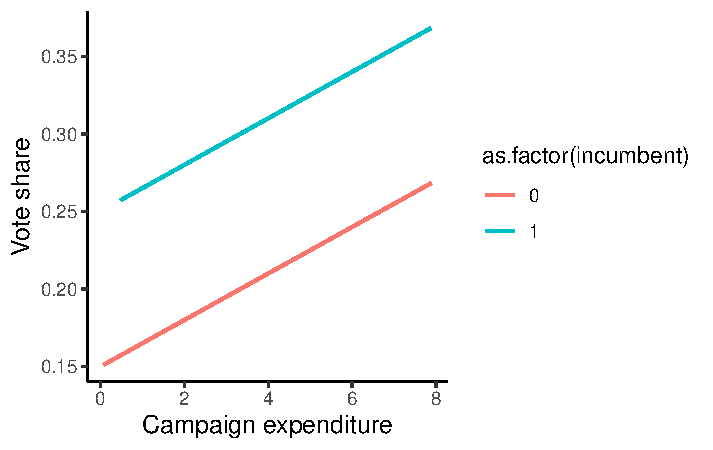
\includegraphics{./../../output/sample_final_incmb.pdf}
\end{center}
\begin{enumerate}
  \item (1 pt) Is $\hat{\beta}_1>0$ or $\hat{\beta}_1<0$, or is it not possible to determine the sign of $\hat{\beta}_1$? Explain your reasoning. 
  \item (1 pt) Is $\hat{\beta}_2>0$ or $\hat{\beta}_2<0$, or is it not possible to determine the sign of $\hat{\beta}_2$? Explain your reasoning. 
  \item (1 pt) What is the interpretation of $\beta_2$? 
\end{enumerate}

\end{enumerate}


\end{document}